\subsection{Closed Loop}
\label{sec:closed_loop}
\begin{figure*}
\centering
%\vspace*{-0.3cm}  
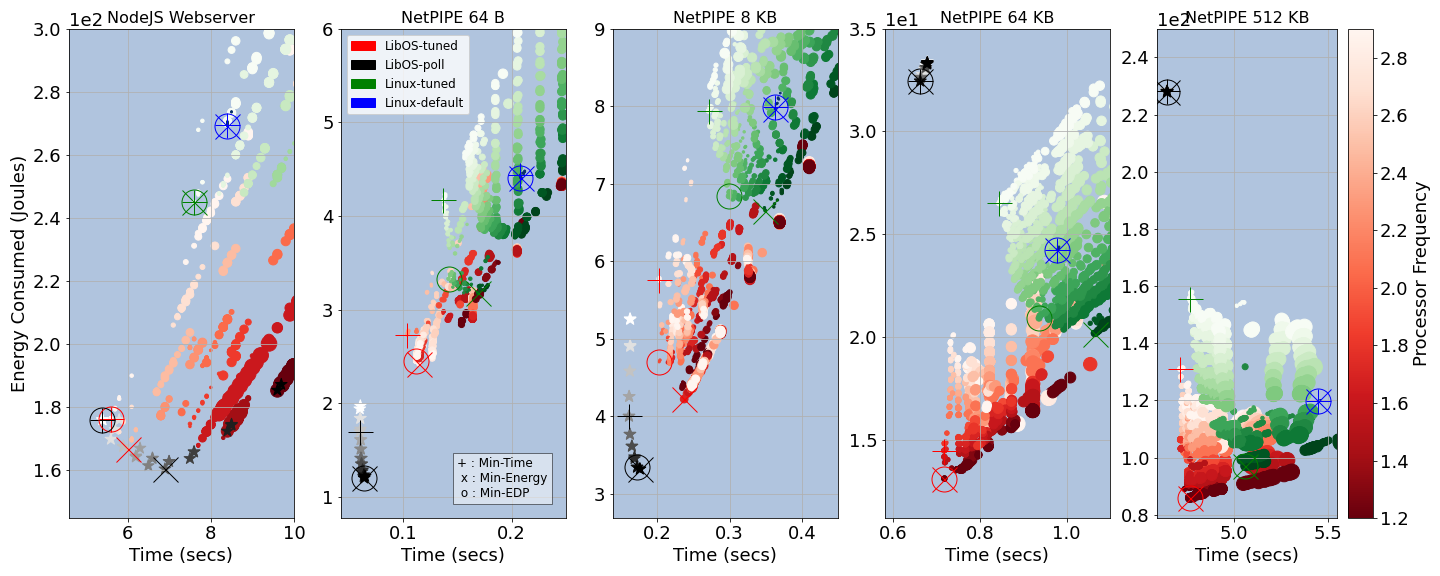
\includegraphics[width=1\textwidth]{figures/closed_loop_overview.png}
\caption[]
%{\small 
{Closed loops.}
\label{fig:closed_loop_overview}
\end{figure*}
\begin{figure*}
\centering
%\vspace*{-0.3cm}  
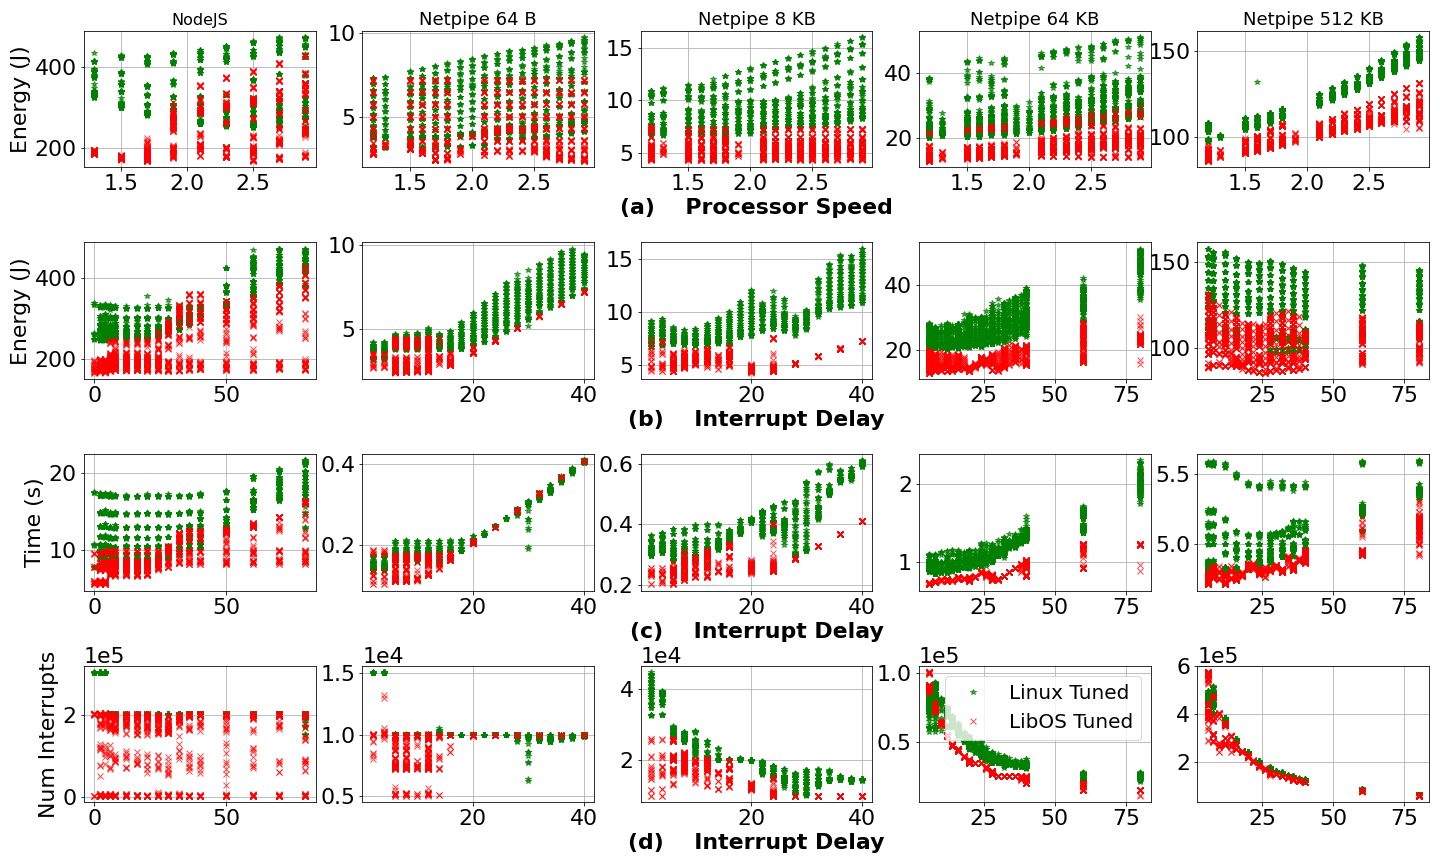
\includegraphics[width=1\textwidth]{figures/closed_detail_1.png}
\caption[]
%{\small 
{Closed loops.}
\label{fig:closed_loop_detail_1}
\end{figure*}
%This approach makes the workloads more predictable and can help smooth out diurnal variations as well~\cite{10.1145/2168836.2168842, 10.1145/2000064.2019527, oldi-study}.
% As pointed out in previous studies of energy proportionality in datacenters, the nature of web-centric applications causes diurnal troughs~\cite{Barroso:2009:DCI:1643608, oldi-study, oldi-pegasus, warehouse-power, energyproportion, WebSearch} and one method with which to increase energy efficiency during these troughs is to maximize the amount of work done, typically under a given energy budget. Figure~\ref{fig:closed_loop_overview} illustrates the set of closed-loop workloads studied in our work, all of the workloads are run in a single core with a single connection, further, they enable us to explore these simple closed-loop examples in detail in settings of computationally intensive (nodejs) and across varying network bandwidth requirements (netpipe). 

Figure~\ref{fig:closed_loop_overview} illustrates the set of closed-loop workloads studied in our work, all of the workloads are run in a single core with a single connection. Netpipe~\cite{snell1996netpipe} involves sending messages of identical size between two systems for a fixed number of iterations. We fix the iteration count at 5000 and show results for a range of message sizes. As message size increases, the workload becomes more network bound; further, linux suffers an additional memory copy from kernel to userspace compared to the libOS. \footnote{We found that the 10 GB link is close to saturation when a message of size greater 700 KB is exchanged.}. NodeJS~\cite{nodejs} consists a JavaScript HTTP Webserver running in side a nodejs runtime. A single client running the \textit{wrk}~\cite{wrk} benchmark\footnote{We modified \textit{wrk} to place a fixed request load of 100K.} sends web requests to the nodejs server for a fixed period of time. The server responds to each request with a small static payload of size 148 bytes. The library OS was ported to support bare-metal nodejs by providing OS interfaces that link with the V8~\cite{v8} JavaScript engine and libuv~\cite{libuv}. 

As datacenter energy use continue to rise~\cite{gupta2020chasing, NLP-energy,warehouse-power}, we believe traditional metrics such as energy-delay-product (EDP), coined from architecture community~\cite{573184,10.1109/40.888701}, should be elevated when studying energy efficiency of applications and the OS. Therefore, we believe it is an apt metric to use when understanding these trade-offs between the system types in a closed loop setting. We use the {\larger[4]\textbf{o}} graphical indicator in the figures below to represent the setting with best (lowest) EDP.

%We believe these set of workloads will help to simplify the complexity which to compare and contrast the effects of slowing down in the four types of systems listed above.

%\subsubsection{Observation-1: Computationally heavy applications exhibits more performance-energy trade-offs}
%Comparing the nodejs and netpipe workloads in figure~\ref{fig:closed_loop_overview}, one can see the differences in trade-offs as processor is slowed. In netpipe, the \textit{vertical-ness} as the datapoints get darker shows that slowing down the processor does not cause an increase in time, whereas the opposite is shown in the nodejs data.

% MIN-TIME linux_default   1 3.0 8.396 269.4
% MIN-TIME linux_tuned     2 2.9 7.599 244.93

% MIN-TIME linux_default 64 1 3.0 0.21 4.44
% MIN-TIME linux_tuned   64 2 2.9 0.14 4.17

% MIN-TIME linux_default 8192 1 3.0 0.36 7.99
% MIN-TIME linux_tuned   8192 8 2.8 0.27 7.94

% MIN-TIME linux_default 65536 1 3.0 0.98 24.25
% MIN-TIME linux_tuned   65536 8 2.9 0.84 26.5

% MIN-TIME linux_default 524288 1 3.0 5.45 119.77
% MIN-TIME linux_tuned   524288 8 2.9 4.77 155.56

% MIN-TIME ebbrt_tuned   4 2.9 5.6 176.11 986.11
% MIN-TIME ebbrt_poll    0 2.9 5.4 176.01 950.1

% MIN-TIME ebbrt_tuned 64 2 2.3 0.1 2.73 0.28
% MIN-TIME ebbrt_poll  64 0 2.5 0.06 1.7 0.1

% MIN-TIME ebbrt_tuned 8192 6 2.9 0.2 5.76 1.16
% MIN-TIME ebbrt_poll  8192 0 2.1 0.16 4.0 0.64

% MIN-TIME ebbrt_tuned 65536 6 1.7 0.72 14.46 10.35
% MIN-TIME ebbrt_poll  65536 6 1.3 0.66 32.45 21.48

% MIN-TIME ebbrt_tuned 524288 6 2.9 4.72 130.94 617.38
% MIN-TIME ebbrt_poll  524288 6 2.7 4.64 228.13 1059.59



% MIN-EDP linux_default 1 3.0 8.4 269.27 2261.6
% MIN-EDP linux_tuned   2 2.9 7.6 244.93 1861.22

% MIN-EDP linux_default 64 1 3.0 0.21 4.41 0.92
% MIN-EDP linux_tuned   64 2 2.1 0.14 3.33 0.47

% MIN-EDP linux_default 8192 1 3.0 0.36 7.99 2.89
% MIN-EDP linux_tuned   8192 10 2.0 0.3 6.84 2.05

% MIN-EDP linux_default 65536 1 3.0 0.98 24.25 23.72
% MIN-EDP linux_tuned   65536 12 1.8 0.94 20.91 19.57

% MIN-EDP linux_default 524288 1 3.0 5.45 119.77 652.63
% MIN-EDP linux_tuned   524288 28 1.2 5.06 97.04 491.22


% MIN-EDP ebbrt_tuned   4 2.9 5.6 176.11 986.11
% MIN-EDP ebbrt_poll    0 2.9 5.4 175.93 949.67

% MIN-EDP ebbrt_tuned   64 6 2.9 0.11 2.45 0.27
% MIN-EDP ebbrt_poll    64 0 1.2 0.06 1.2 0.08

% MIN-EDP ebbrt_tuned 8192 2 1.9 0.2 4.7 0.95
% MIN-EDP ebbrt_poll  8192 0 1.3 0.17 3.34 0.57

% MIN-EDP ebbrt_tuned 65536 6 1.2 0.72 13.07 9.37
% MIN-EDP ebbrt_poll  65536 6 1.3 0.66 32.45 21.48

% MIN-EDP ebbrt_tuned 524288 26 1.2 4.77 85.94 409.68
% MIN-EDP ebbrt_poll  524288 6 1.5 4.65 227.86 1058.57

% find configurations in which the OS interacts with slowing down to improve both time and energy. 
\subsubsection{Speeding up to save energy}
%% relation between quiescent and time to do work
As discussed in closed loop workload analysis in section~\ref{sec:workflow:closed_loop}, figures~\ref{fig:closed_loop_overview} demonstrates the correlation that minimizing the time to finish the work and also results in most energy savings. One mechanism to reduce time across all the closed loop workloads and system types is to speed up interrupt delays (set a low interrupt delay value) as shown in figure~\ref{fig:closed_loop_detail_1}(c); while slow down processor does cause fluctuations in time for each interrupt delay value, the overall trend is low interrupt delay results in lowest time. By reducing time, one also minimizes energy as shown in figure~\ref{fig:closed_loop_detail_1}(b). For nodejs and netpipe 64B, we found setting a low interrupt delay (2$\mu$s)also results in the lowest EDP, this due to the lightweight nature of the payloads themselves (under a single MTU). However, as the payload sizes increase (to 8KB, 64KB, and 512KB), we found the interrupt delay value that yields best EDP also become larger, up to 28$\mu$s. A 10 GbE NIC, assuming no network jitter and switching cost, can transmit at an optimal rate of 1250 bytes/$\mu$s. With larger payload sizes, one can imagine portions of its payload being transmitted over the wire and processed by software asynchronously. The interrupt delay value that yields best EDP is effectively indicating an optimal configuration with which the software should pace packet processing and save energy by sleeping during the its quiescent periods. By modulating interrupt delay, Linux-tuned improves its EDP over Linux-default by 21\%-80\%. Due to the OS path length efficiency of the libOS (figure~\ref{fig:closed_loop_detail_1}), we find the libOS uses fewer instructions even in computationally heavy workloads such as nodejs (7.2\%), this efficiency coupled with a custom interrupt delay enables the libOS to achieve up to 2X better EDP.

%One can also notice the wider variation in time for nodejs in figure~\ref{fig:closed_loop_detail_1}(c), this is mainly the result of greater performance-energy trade-offs that occur in a computationally bound application.

\subsubsection{Slow-to-stay-busy effect}
In the library OS, we find slowing down of the processor results in a new energy efficient state which we term \textit{slow-to-stay-busy}. In figure~\ref{fig:closed_loop_detail_1}(d), one can see that in both nodejs and netpipe 64 B, for various interrupt delay values, the number of interrupts can be lowered by up to 90\%. Upon closer examining the data, we find slowing down of the processor actually causes this decrease in number of interrupts. The reason for this behavior in the library OS can be seen in figure~\ref{fig:timeline}; the physical transmission of OS reply packets by the network driver can occur in parallel with the un-winding of the stack back to the nodejs application and then down (again) to the network receive function to check for incoming packets. It is during this un-winding code path where slowing down of the processor actually results in a slow-to-stay-busy state where by the time the un-wind has reached the network receive function (again), the response to the initial transmitted packet has already arrived, therefore the the software is able to skip another hardware interrupt in order to effectively stay busy and process this new reply packet. This scenario only occurs in the library OS due to the run-to-completion nature of its OS structure.
%what are configurations where this doesn't occur??

% MIN-TIME linux_default 65536 1 3.0 0.98 24.25 23.72
% MIN-TIME linux_tuned 65536 8 2.9 0.84 26.5 22.37
% MIN-TIME ebbrt_tuned 65536 6 1.7 0.72 14.46 10.35
% MIN-TIME ebbrt_poll 65536 6 1.3 0.66 32.45 21.48

% MIN-TIME linux_default 524288 1 3.0 5.45 119.77 652.63
% MIN-TIME linux_tuned 524288 8 2.9 4.77 155.56 741.87
% MIN-TIME ebbrt_tuned 524288 6 2.9 4.72 130.94 617.38
% MIN-TIME ebbrt_poll 524288 6 2.7 4.64 228.13 1059.59

\subsubsection{Trade-offs in library OS polling}
 For nodejs, LibOS-poll results in a better (lower) EDP than LibOS-tuned by 4\%, partially this is due to nodejs' application code is already warmed up by containing a polling loop to check for inbound packets. For netpipe 64B and 8KB, EDP by polling is more effective by 1.6X and 3.3X respectively. We hypothesize this is due to the smaller payload sizes, therefore getting the work done the fastest results in the lowest energy use. As payload size increases, the workload becomes more network bound, therefore polling actually results in worse EDP by up to 2X. We find at these larger payload sizes, polling only reduced time by around 10\%, however energy consumption was over 2X worse.

%% Vertical behavior of Netpipe 64 KB and 512 KB??